\documentclass[12pt, french]{article}

\usepackage{fancyhdr, fancybox, lastpage,mhchem, mathrsfs, tikz}
\usepackage[most]{tcolorbox}
\usepackage[a4paper, margin={0.3in, .75in}]{geometry}
\usepackage{wrapfig}
\pagestyle{fancy}
\renewcommand\headrulewidth{1pt}
\renewcommand\footrulewidth{1pt}
\fancyhf{}
\rhead{ \em{Zakaria Haouzan}}
\lhead[C]{\em{2ème année baccalauréat Sciences Physiques}}
\chead[C]{}
\rfoot[C]{}
\lfoot[R]{}
\cfoot[]{\em{Page \thepage / \pageref{LastPage}}}


\newtcolorbox{Box2}[2][
enhanced, 
    breakable,
]{
                lower separated=false,
                colback=white,
colframe=white!20!black,fonttitle=\bfseries,
colbacktitle=white!30!gray,
coltitle=black,
enhanced,
attach boxed title to top left={yshift=-0.1in,xshift=0.15in},
title=#2,#1}


\begin{document}
\begin{center}
   \shadowbox {\bf{Mouvement des satellites et planètes }
 }

\end{center}

\vspace{-0.2cm}
%%_________________________Exercice ! :"_________________________Exercice
   \begin{Box2}{Exercice 1 : Le pigeon bleu.}

	\begin{wrapfigure}[4]{r}{0.26\textwidth}
  \begin{center}
	  \vspace{-0.6cm}
	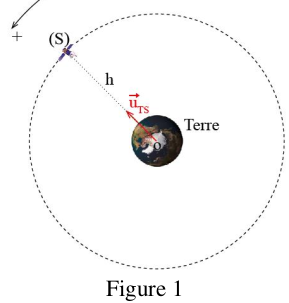
\includegraphics[width=0.26\textwidth]{./ex_00.png}
  \end{center}
\end{wrapfigure}

\emph{ Le pigeon bleu est un satellite artificiel marocain assurant le contrôle des frontières
géographiques du royaume et les télécommunications. Il a été instauré par des
experts du centre royal de télédétection spatiale en collaboration avec experts
internationaux.}

\emph{Le pigeon bleu a été mis en orbite le 10 décembre 2001 à une altitude h du sol. \\Ce
satellite artificiel (S) effectue environ 14 tours autours de la terre par jour. }

\textbf{Données} : 

\begin{itemize}
	\item On assimile l’orbite de (S) à un cercle de centre O, et on étudie son mouvement
dans le repère géocentrique.
\item La Terre est considérée comme une sphère à répartition sphérique de masse.
\item  On néglige les dimensions de (S) devant sa distance au centre de la Terre.

\item La valeur de la constante de gravitation universelle : $G = 6,67.10^{-11}$ (SI) ;
\item  La valeur du rayon de la Terre : $r_T = 6350 km$ ;
\item  La valeur de l’intensité de pesanteur à la surface
	de la Terre : $g_0 = 9,8 m.s^{-2}$ ;
\item La valeur de la période de rotation de la Terre
autour de son axe polaire : $T = 86164 s$ ;
\item La valeur de l’altitude : $h = 1000 km$ ;
\item $\vec{u_TS}$ : Vecteur unitaire dirigé de O vers S.

\end{itemize}

\begin{enumerate}

	\item Recopier le schéma de la figure 1, et représenter dessus le vecteur vitesse $\vec{V_S}$ du
satellite artificiel, et le vecteur force d’attraction universelle modélisant l’action
de la Terre sur (S).

\item Donner l’expression vectorielle de la force d’attraction universelle modélisant
l’action de la Terre sur (S).

\item Ecrire dans le repère de Freinet, l’expression du vecteur accélération du
mouvement de (S).

\item Par application de la 2ème loi de Newton sur le mouvement du centre de gravité
du satellite (S) :
\begin{enumerate}
	\item Montrer que le mouvement de (S) est circulaire uniforme.
	\item Ecrire l’expression de $V_S$ en fonction de $g_0$, $r_T$, et $h$. Calculer sa valeur.
\end{enumerate}

\item Montrer que la masse de la terre est : $M_T = 6.10^{24} kg$.
\item Montrer que le satellite artificiel n’apparait pas immobile par rapport à un
Un autre satellite artificiel (S’) tourne autour de la Terre avec une vitesse
angulaire $\omega$, et apparait immobile par rapport à un observateur terrestre.
Le satellite (S’) envoie à la terre des photos utilisées dans les prévisions météo.
\begin{enumerate}
	\item Montrer que : $\omega^2.(r_T + z)^3 = Cte$ où est la distance séparant le sol terrestre du
satellite (S’).
\item  Trouver la valeur de z.
\end{enumerate}


\end{enumerate}


   \end{Box2}


%%_________________________Exercice !2 :"_________________________Exercice
\begin{Box2}{Exercice 2 :le mouvement de Jupiter autour du soleil. }
   % \begin{wrapfigure}[1]{r}{0.32\textwidth}
  %\begin{center}
	  %\vspace{-0.6cm}
	%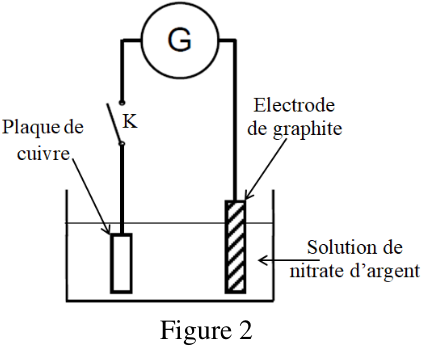
\includegraphics[width=0.32\textwidth]{./ex_01.png}
  %\end{center}
%\end{wrapfigure}
Le but de cet exercice est d’étudier le mouvement de Jupiter autour du soleil, et de
déterminer quelques grandeurs physiques caractérisant cette planète.
\textbf{Données : }
\begin{itemize}

	\item Masse du soleil : $M_S = 2.10^{30} kg$ ;
	\item Constante d’attraction universelle : $G = 6,67.10^{-11}$ (SI) ;
	\item Période de révolution de Jupiter autour du soleil : $T_J = 3,74.10^8 s$ ;
\end{itemize}
On considères que le soleil et Mars sont à répartitions sphériques de masses, et on
note la masse de Jupiter $M_J$.

On néglige les dimensions de la planète Jupiter devant la distance qui la sépare du
centre du Soleil, ainsi que les forces qui lui sont appliquées devant la force
d’attraction universelle entre elle et le Soleil.

\textbf{\underline{1- Détermination du rayon orbital de Jupiter et sa vitesse : }}

On considère que le mouvement de Jupiter dans le repère héliocentrique est circulaire
de rayon orbital r.

\begin{enumerate}

	\item Ecrire en fonction de $M_J$, $M_S$, $G$, et $r$, l’expression de l’intensité de la force
de gravitation universelle exercée par le Soleil sur Jupiter.
	\item En appliquant la deuxième loi de Newton :
		\begin{enumerate}

			\item Ecrire les expressions des composantes du vecteur accélération dans le
repère de Freinet, et déduire que le mouvement de Jupiter est
circulaire uniforme. 
\item Montrer que la troisième loi de Kepler s’écrit $\frac{T_J^2}{r^3} = \frac{4.\pi^2}{G.M_S}$

		\end{enumerate}
	\item S’assurer que $r \approx 7,8.10^{11}m$.
	\item  Déterminer la valeur de la vitesse V de révolution de Jupiter autour du
soleil. 
\end{enumerate}

\textbf{\underline{2- Détermination de la masse de Jupiter : }}

On considère que la lune "Io" l’un des satellites découvert par Galilée, est en
mouvement circulaire uniforme à une distance $r’ = 4,2.10^8 m$ du centre de Jupiter.
La période de ce mouvement est $T_I = 1,77 jours$.
(On néglige les dimensions de Io devant les autres dimensions, ainsi que les forces qui
lui sont appliquées devant la force d’attraction universelle entre lui et Jupiter).

En étudiant le mouvement de Io dans un repère d’origine confondu avec le centre de
Jupiter et supposé galiléen, \textbf{déterminer la masse $M_J$ de Jupiter.}
\end{Box2}

%\begin{Box2}{Exercice 3 :Etude du mouvement d’une particule chargée dans un champ magnétique  }
%\end{Box2}
	%\vspace{-0.8cm}


%\begin{Box2}{Exercice 4 :Les toboggans}

%\end{Box2}




%\begin{Box2}{Exercice 5 : Etude du mouvement du centre de gravité d’une balle. }
%%\begin{wrapfigure}[3]{r}{0.33\textwidth}
	%%\vspace{-0.8cm}

%\end{Box2}


%\begin{center}
   %\Large{ \em{Exercices Supplémentaires}}
%\end{center}

%\vspace{-0.8cm}

%%%_________________________Exercice ! 3:"_________________________Exercice
%\begin{Box2}{Exercice 6:Etude du mouvement d’une balle de golf dans le champ de pesanteur uniforme }
%%\begin{wrapfigure}{r}{0.4\textwidth}
 %%\end{wrapfigure}

%\end{Box2}

%%_________________________Exercice 4 : _________________________Exercice
%\begin{Box2}{Exercice 7 :Le ski }
   %% \begin{wrapfigure}[12]{r}{0.5\textwidth}

%%\end{wrapfigure}


%\end{Box2}
\begin{center} \emph{\textbf{“The physical universe and its buzzing machinery, its fantastical scenery.”}}
\end{center}

%\vspace{-0.6cm}
%%%_________________________Exercice 5 : _________________________Exercice
%\begin{Box2}{Exercice 4 : }
   %% \begin{wrapfigure}[14]{r}{0.5\textwidth}
  %%\begin{center}
	  %%\vspace{-0.6cm}
	%%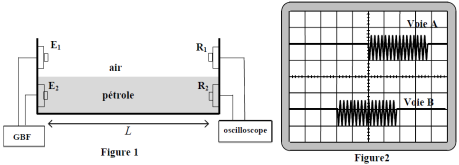
\includegraphics[width=0.5\textwidth]{./img/ex5.png}
  %%\end{center}
%%\end{wrapfigure}

%4

%\end{Box2}

%\begin{Box2}{Exercice 5 : }

%44
%\end{Box2}


%\begin{Box2}{Exercice 6 : }


	%\end{Box2}


%\begin{Box2}{Exercice 7 : }
%\end{Box2}
\end{document}
